%%% BEN 7.5' %%%

\section{Hyperfeinstrukturspektrum}
\subsection{Aufbau}


\begin{frame}
\frametitle{Aufbau: Bestimmung der Scanrate des Lasers}

\setbeamerfont{myfont}{size*=80}
\usebeamerfont{myfont}
\begin{figure}
    \centering
    \def\svgwidth{\textwidth}
    \input{../img/aufbauEtalon.pdf_tex}
    \caption{Aufbau zur Bestimmung der Scanrate des Lasers mit Hilfe des Etalons.}
\end{figure}



\end{frame}

\begin{frame}
\frametitle{Aufbau: Hyperfeinstrukturspektrum}

\setbeamerfont{myfont}{size*=80}
\usebeamerfont{myfont}
\begin{figure}
    \centering
    \def\svgwidth{\textwidth}
    \input{../img/aufbauHFSSpektrum.pdf_tex}
    \caption{Aufbau zur Messung des Hyperfeinstrukturspektrums.}
\end{figure}
\usebeamerfont{standard}


\begin{itemize}
  \item \textbf{Rubidiumzelle:} Füllung mit $^{85}$\!Rubidium\,+\,$^{87}$\!Rubidium (T$_\text{m}=39^\circ$C)
  und Puffergas Krypton ($p=1.5$\,mbar)
   
\end{itemize}

\end{frame}



\begin{frame}
\frametitle{Foto von Aufbau}

hier ein echtes foto

\end{frame}



\subsection{Auswertung}
\begin{frame}
\frametitle{Auswertung: Bestimmung der Scanrate des Lasers}
\begin{figure}
    \centering
    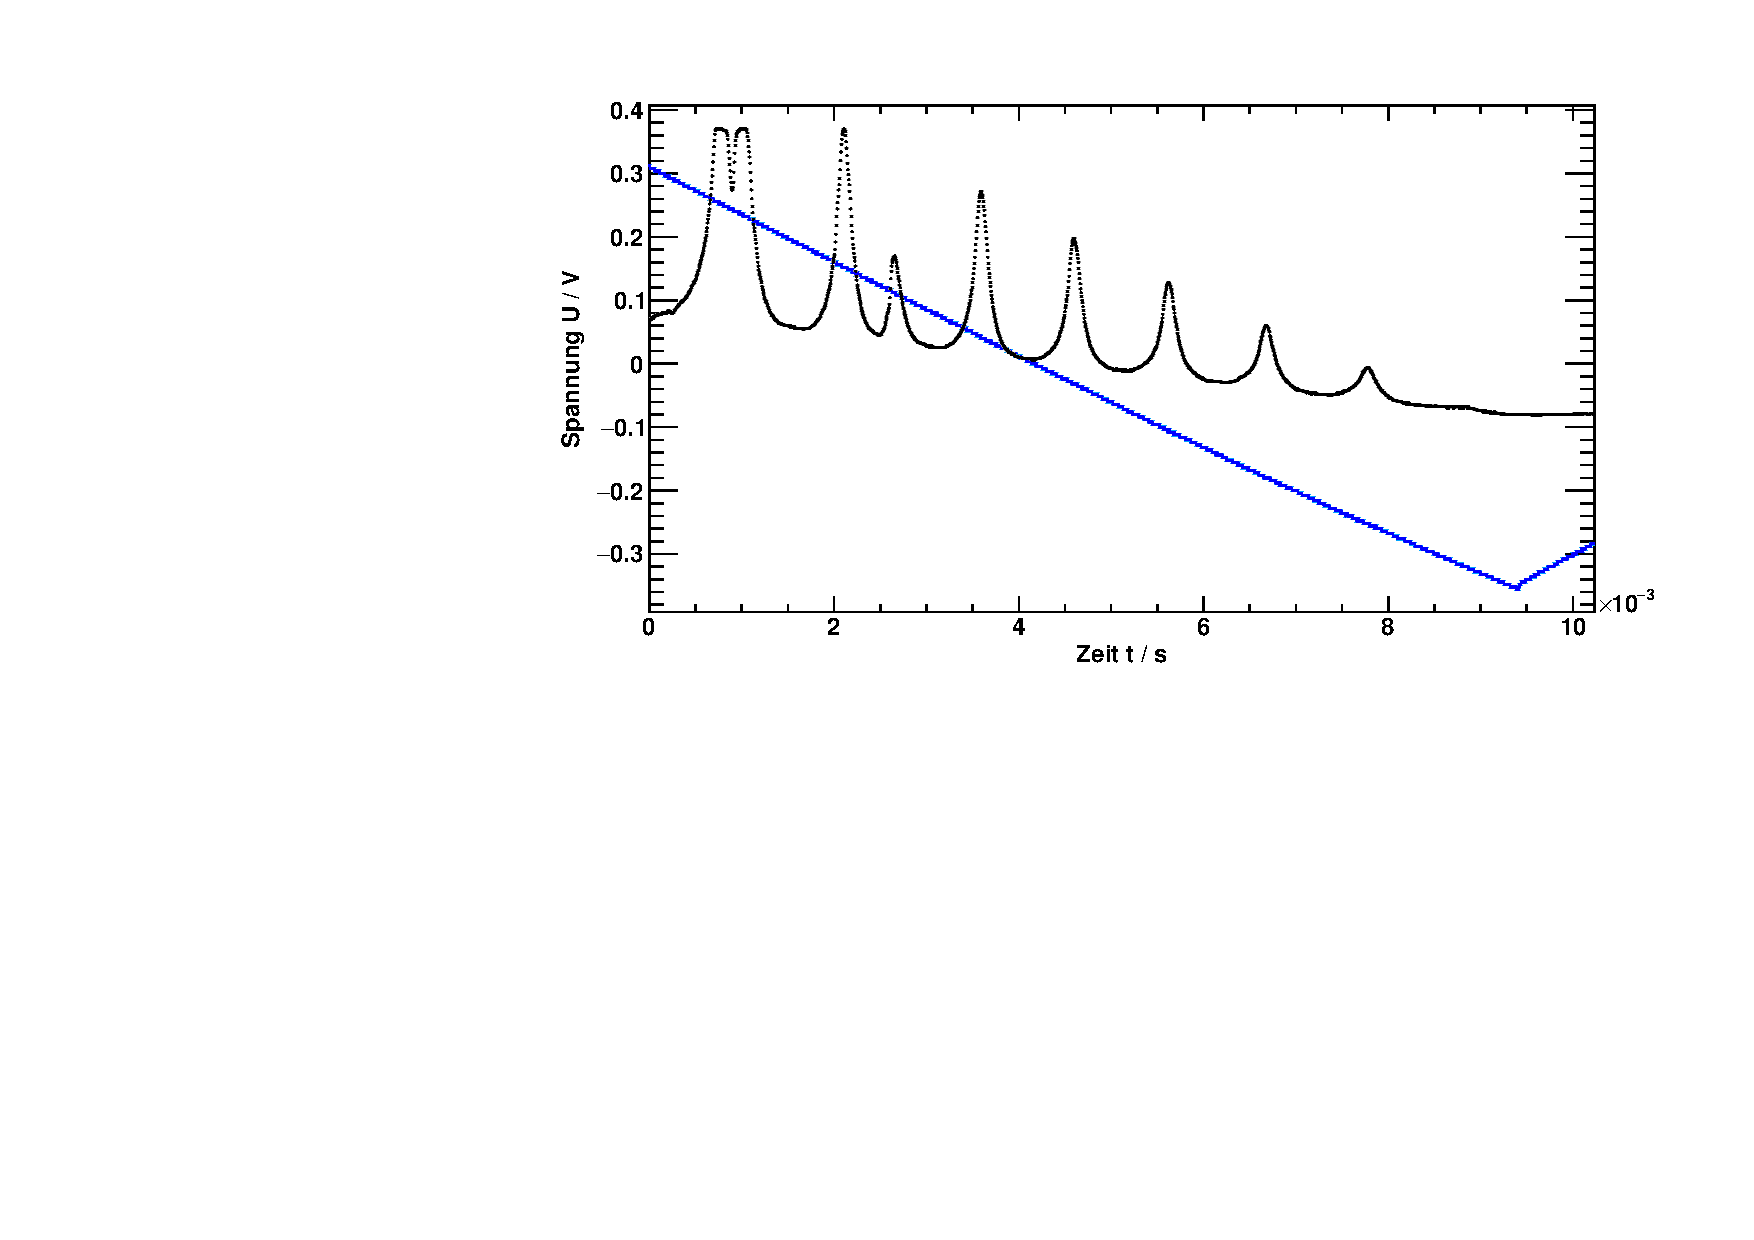
\includegraphics[width=\textwidth]{../img/down-etalon_zoom.pdf} % TODO Achsenbeschriftung
    \caption{Peaks des Etalonspektrums auf fallender Flanke.}
\end{figure}
\end{frame}

%\begin{frame}
%\frametitle{Auswertung: Bestimmung der Scanrate des Lasers}
%\begin{itemize}
%    \item<1-> Fit der Peaks mit Breit-Wigner-Verteilung und linearem Untergrund
%    \begin{equation*}
%        U_\text{ph}(t) = a_\text{ph} + b_\text{ph} \cdot t + \frac{A}{\pi} \frac{s}{s^2 + (t-x)^2}
%    \end{equation*}
%    Amplitude $A$, Zentrum $x$ und Breiteparameter $s$
%    \item<2-> Fit der Spannung für Lasermodulation mit Gerade
%\end{itemize}
%\end{frame}

\begin{frame}
\frametitle{Auswertung: Bestimmung der Scanrate des Lasers}
\begin{figure}
    \centering
    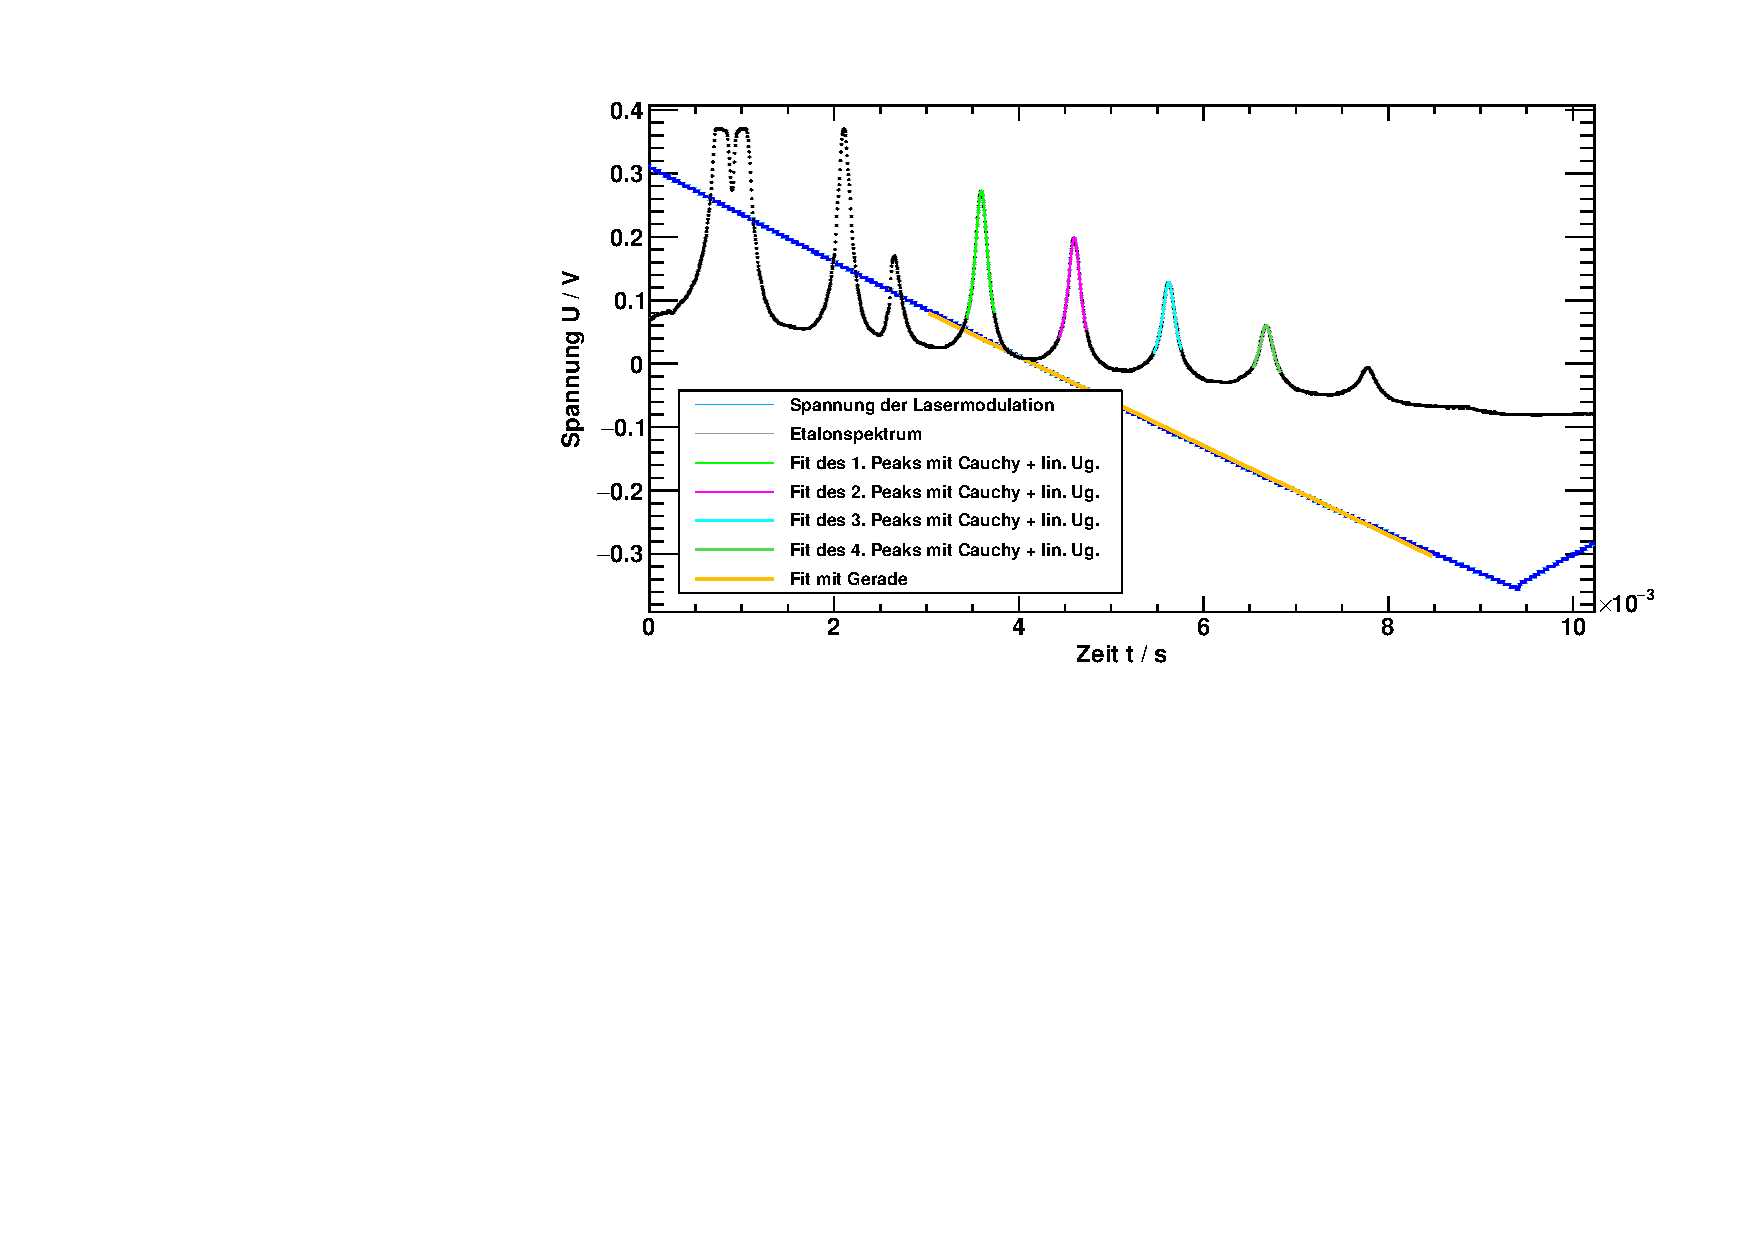
\includegraphics[width=\textwidth]{../img/down-etalon_zoom_fit.pdf}
    \caption{Fit mit Breit-Wigner-Kurven.}
\end{figure}
\end{frame}

\begin{frame}
\frametitle{Auswertung: Bestimmung der Scanrate des Lasers}
  \begin{figure}[H]
      \centering
      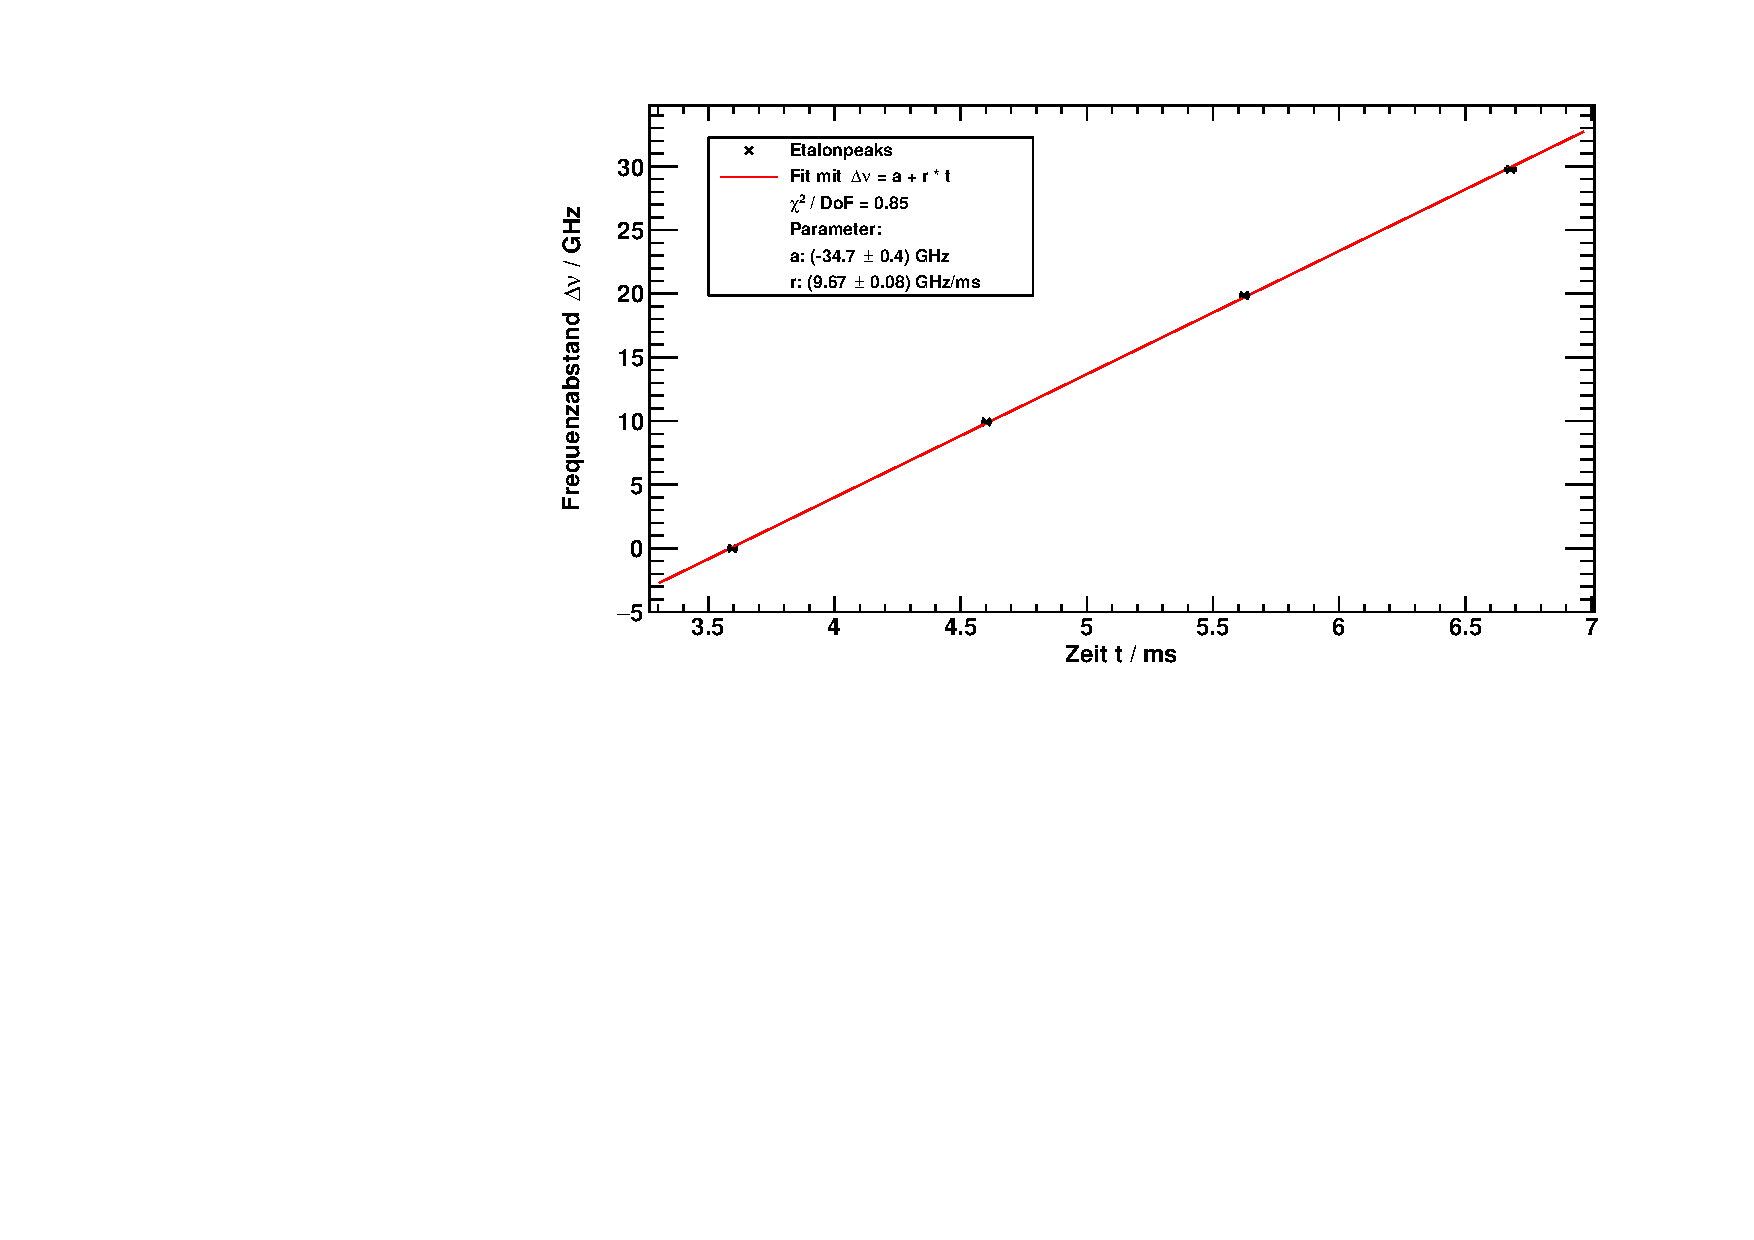
\includegraphics[width=\textwidth]{../img/down-etalon_zoom-etalon_calibration.pdf}
      \caption{Frequenzdifferenz der Etalonpeaks aufgetragen gegen ihre Positionen.}
  \end{figure}
\end{frame}

\begin{frame}
\frametitle{Auswertung: Bestimmung der Scanrate des Lasers}
Fit mit
\begin{equation*}
    \Delta \nu(t) = a + r \cdot t
\end{equation*}
Scanrate $r$ des Lasers
\begin{equation*}
    r = (9.47 \pm 0.08)\,\frac{\text{GHz}}{\text{ms}}
\end{equation*}
\end{frame}

\begin{frame}
\frametitle{Auswertung: Hyperfeinstruktur-Übergänge}
\begin{figure}[H]
    \centering
    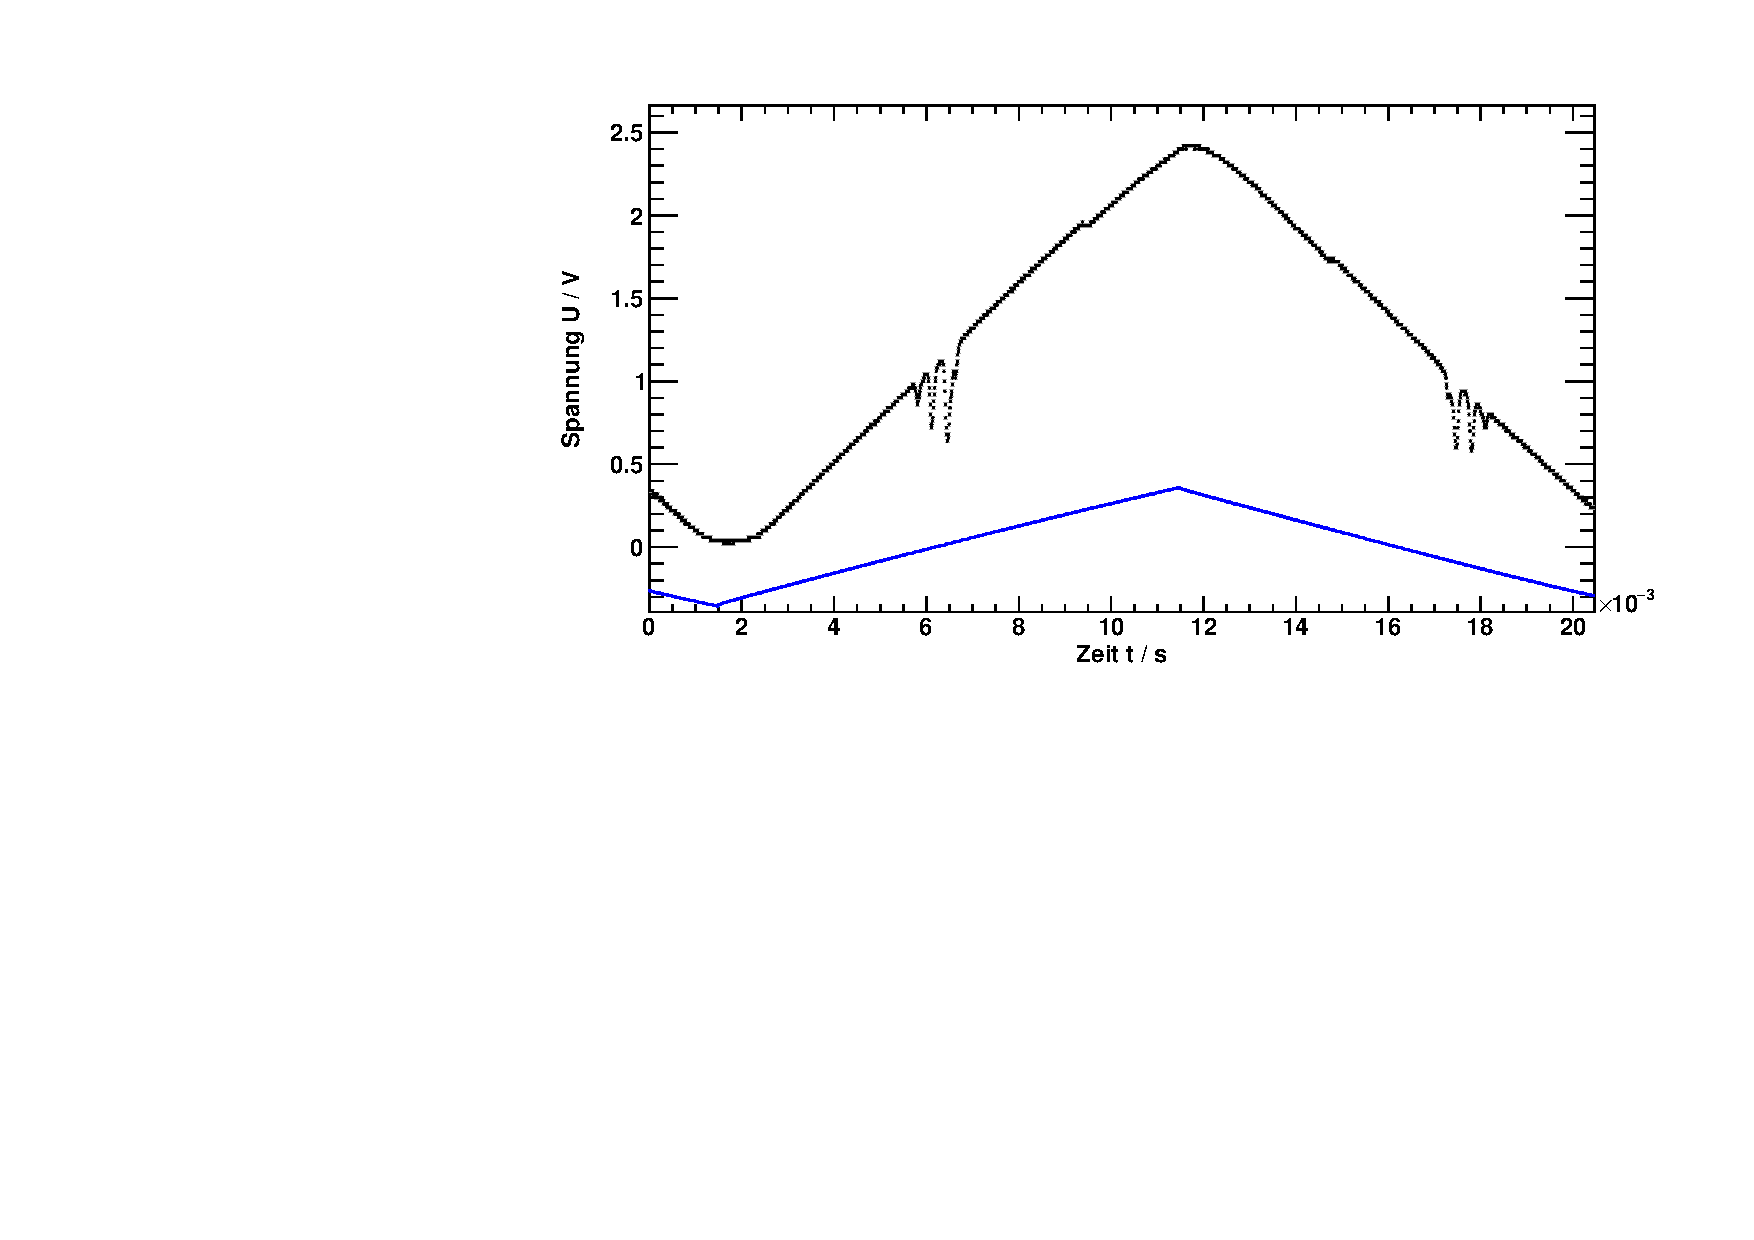
\includegraphics[width=\textwidth]{../img/down-hfs.pdf}
    \caption{Hyperfeinstrukturspektrum von Rubidium.}
\end{figure}
\end{frame}

\begin{frame}
\frametitle{Auswertung: Hyperfeinstruktur-Übergänge}
\begin{figure}[H]
    \centering
    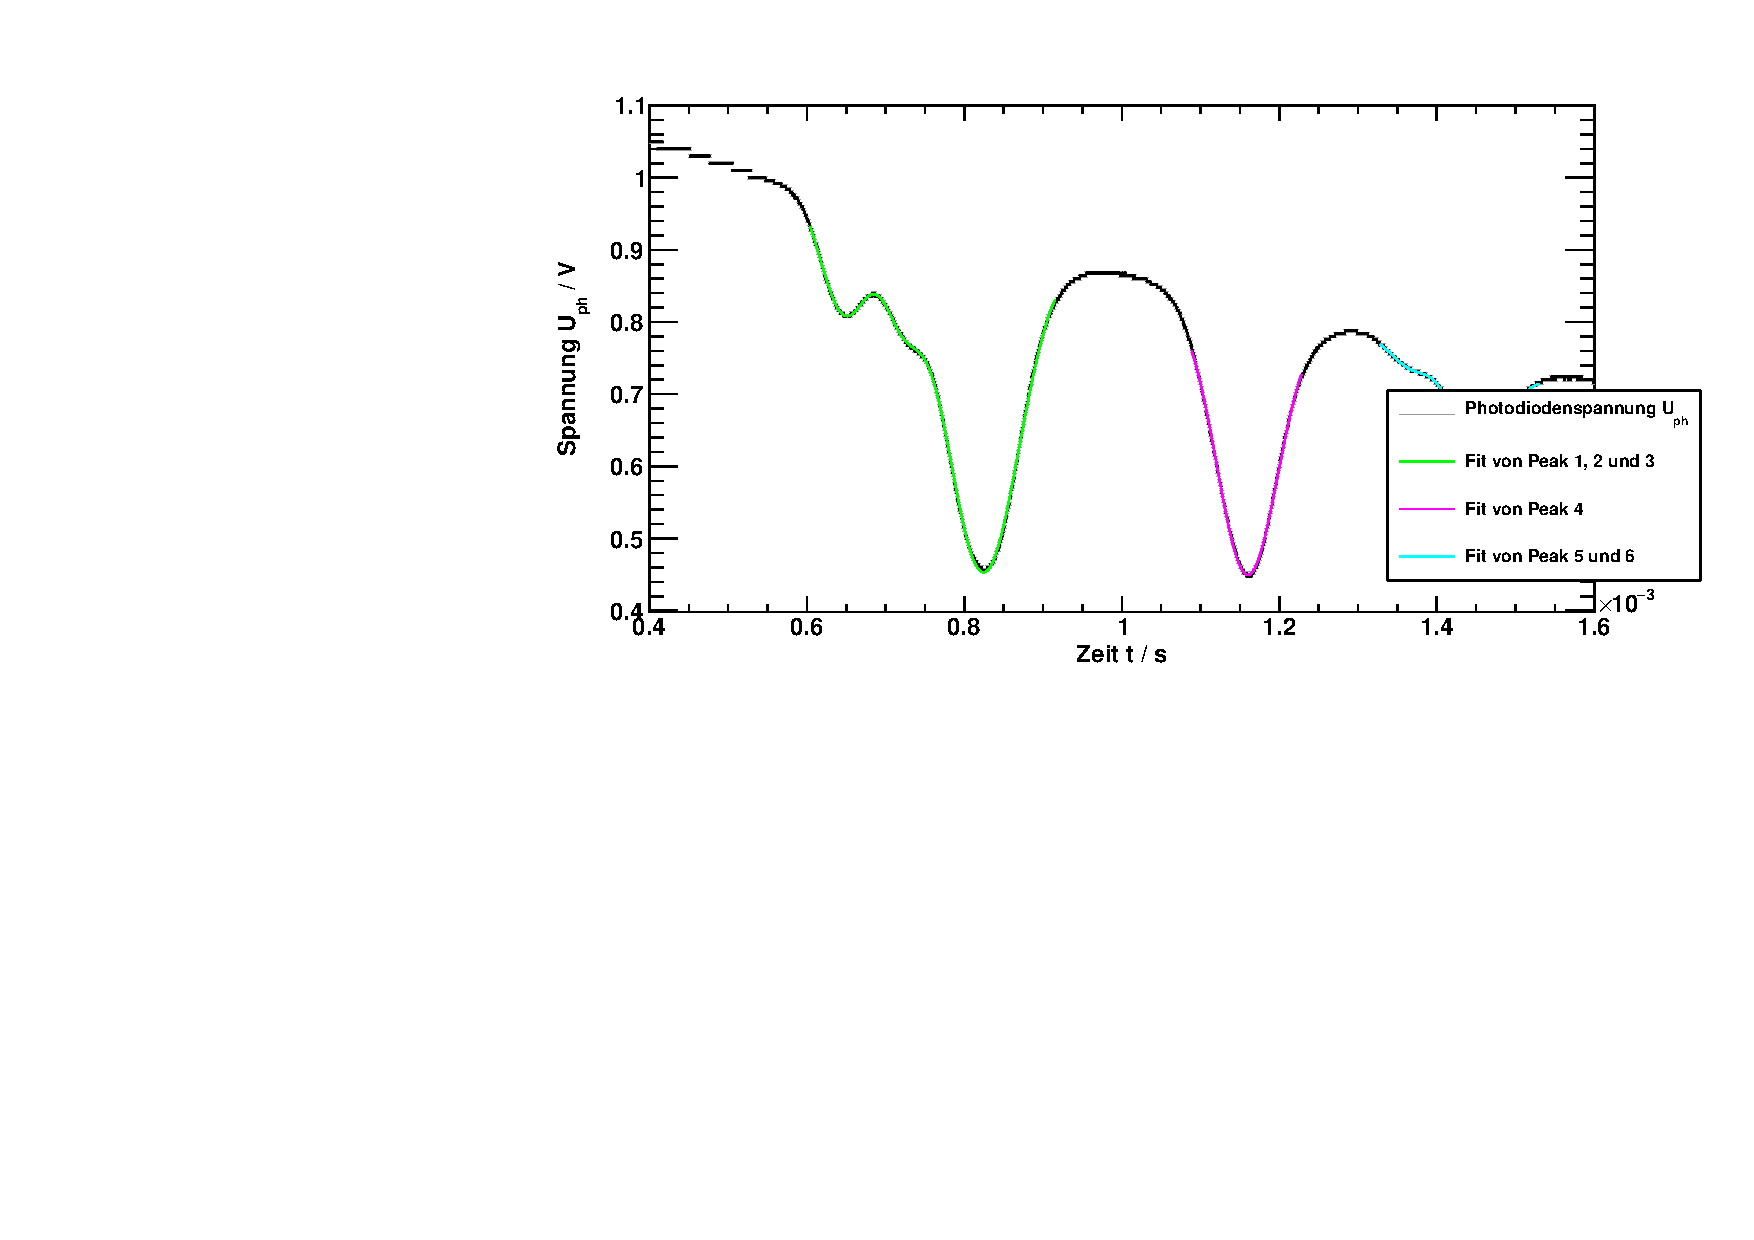
\includegraphics[width=\textwidth]{../img/down-hfs_zoom_fit.pdf}  % TODO Legend
    \caption{Hyperfeinstrukturspektrum von Rubidium mit Fit von überlagerten Gauß-Kurven.}
\end{figure}
\end{frame}

\begin{frame}
\frametitle{Auswertung: Hyperfeinstruktur-Übergänge}
\begin{equation*}
    \Delta \nu_i = r \cdot \left( \mu_i - \mu_3 \right)
\end{equation*}
\end{frame}

\begin{frame}
\frametitle{Auswertung: Hyperfeinstruktur-Übergänge}
\begin{figure}
\begin{center}
    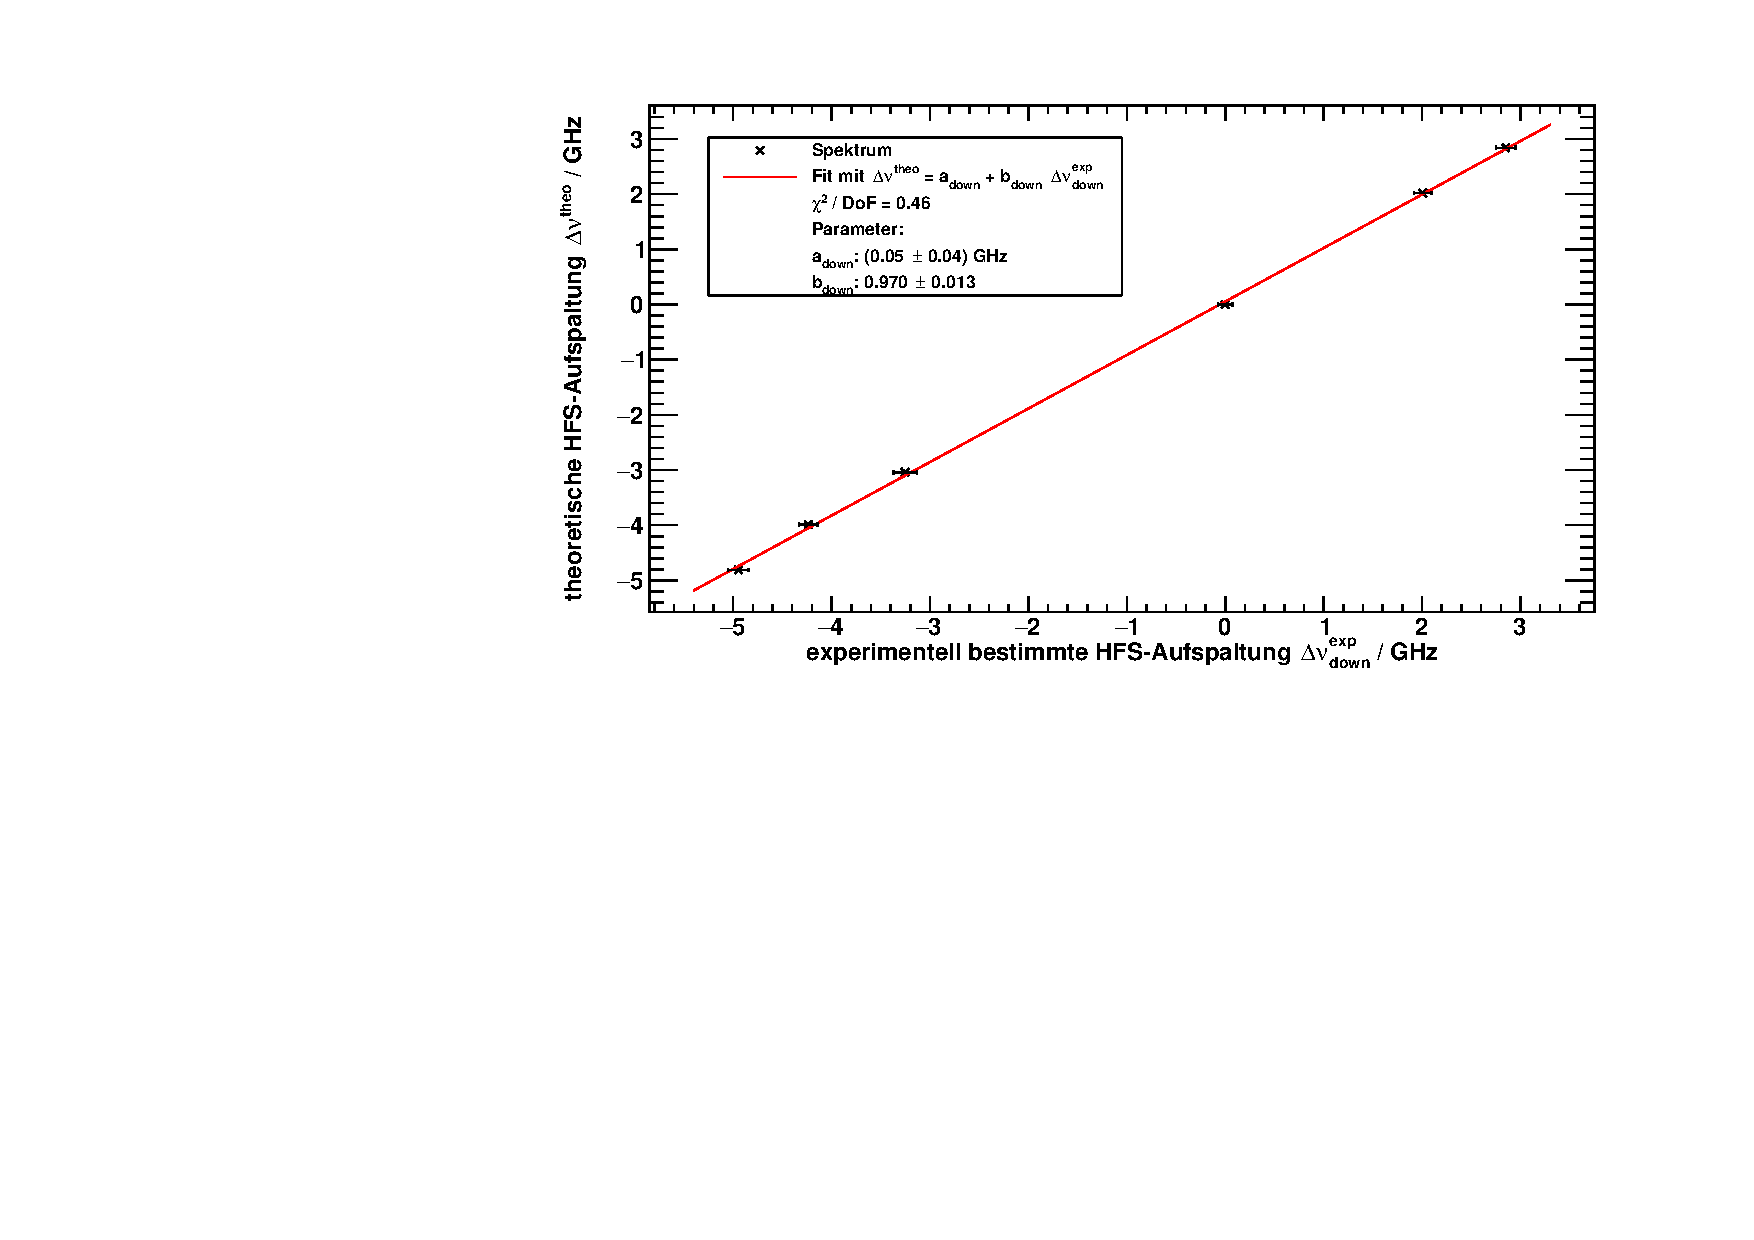
\includegraphics[width=\textwidth]{../img/down-spectrum.pdf}
    \caption{Vergleich des auf der fallenden Flanke gemessenen Hyperfeinstrukturspektrums mit den theoretischen Werten.}
\end{center}
\end{figure}
\end{frame}

\begin{frame}
\frametitle{Auswertung: Hyperfeinstruktur-Übergänge}
\begin{itemize}[<+->]
    \item Fit mit
    \begin{equation*}
        \Delta \nu^\text{theo} = a + b \cdot \Delta \nu^\text{exp}_\text{down}
    \end{equation*}
    \item Ergebnis
    \begin{equation*}
        \begin{split}
            & a = (0.05 \pm 0.04)\,\text{GHz} \\
            & b = 0.970 \pm 0.013
        \end{split}
    \end{equation*}
    \item Möglicher Fehler: Etalon im Strahlengang verkippt
    \begin{itemize}[<+->]
        \item[$\Rightarrow$] Verkleinerung des freien Spektralbereichs
        \item[$\Rightarrow$] Vergrößerung der Abstände der Peaks
        \item[$\Rightarrow$] kleinere Steigung der Vergleichsgeraden
    \end{itemize}
\end{itemize}
\end{frame}

\begin{frame}
\frametitle{Auswertung: Berechnung der Intervallkonstanten $A$}
TODO Bild Termschema ohne Zeeman %TODO Termschema
\end{frame}

\begin{frame}
\frametitle{Auswertung: Berechnung der Intervallkonstanten $A$}
\begin{figure}
    \centering
    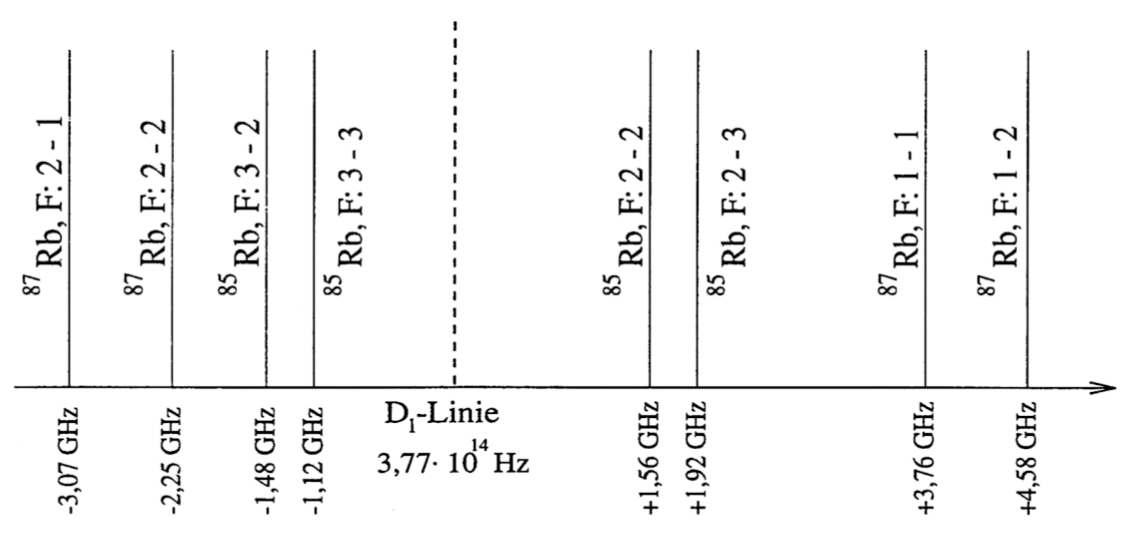
\includegraphics[width=\textwidth]{../img/HFSspect_theo.png}
    \caption{Spektrallinien der Hyperfeinstruktur des ${}^2\text{S}_{1/2}$\,-\,${}^2\text{P}_{1/2}$\,-\,Übergangs
    von \rb{85} und \rb{87}.}  % TODO Inkscape oder ref
\end{figure}
\end{frame}

\begin{frame}
\frametitle{Auswertung: Berechnung der Intervallkonstanten $A$}
\begin{equation*}
    \Delta E = \Delta \nu h = A (F + 1)
\end{equation*}
\begin{table}
\caption{Errechnete HFS-Intervallkonstanten $A$ für das ${}^2\text{S}_{1/2}$ Niveau von \rb{85} und für das ${}^2\text{S}_{1/2}$- und ${}^2\text{P}_{1/2}$ Niveau von \rb{87}.}
\begin{center}
\begin{tabular}{|c|c|c|c|}
  \hline
  Isotop / Feinstruktur & $A^\text{Lit.}$ / \textmu eV & $A^\text{exp}$ / \textmu eV & $s_{A^\text{exp}}$ / \textmu eV \\ \hline
  \rb{85}: ${}^2\text{S}_{1/2}$ & 4.185 & 4.47 & 0.14 \\ \hline
  \rb{87}: ${}^2\text{S}_{1/2}$ & 14.13 & 14.49 & 0.14 \\ \hline
  \rb{87}: ${}^2\text{P}_{1/2}$ & 1.692 & 1.61 & 0.14 \\ \hline
\end{tabular}
\end{center}
\label{tab:hfs:intervalconsts}
\end{table}
\end{frame}